% ==========================================
% ФАЙЛ: p4.tex
% БЛОК БИЛЕТОВ 16-20 (По официальному списку вопросов)
% ==========================================

% --- Вопрос 16 ---
\examquestion{16}{Линейность определенного интеграла}
{Сформулируйте и докажите теорему о линейности определенного интеграла Римана через предел интегральных сумм $\sigma(f,T,\xi)$. Покажите, как свойства предела суммы и выноса константы для конечных сумм переносятся на бесконечный предел при мелкости разбиения $\lambda(T)\rightarrow0$. Докажите из линейности свойство сохранения знака интеграла.}

\paragraph{Суть на пальцах}
Интеграл — это площадь фигуры. Свойство линейности означает две интуитивно понятные вещи:
1. Если график функции вытянуть в высоту в 2 раза (умножить на константу), то и площадь под ним увеличится ровно в 2 раза.
2. Если поставить одну фигуру "на плечи" другой (сложить функции $f+g$), то их общая площадь будет равна сумме площадей каждой фигуры по отдельности. 

\paragraph{1. Формулировка и доказательство теоремы о линейности}
Пусть функции $f(x)$ и $g(x)$ интегрируемы на отрезке $[a, b]$ ($f, g \in \mathcal{R}[a, b]$). Тогда для любых констант $\alpha, \beta \in \mathbb{R}$ их линейная комбинация $(\alpha f(x) + \beta g(x))$ также интегрируема на $[a, b]$, причем:
$$ \int_a^b (\alpha f(x) + \beta g(x)) dx = \alpha \int_a^b f(x) dx + \beta \int_a^b g(x) dx $$

\begin{proof}
Зададим произвольное разбиение $T$ отрезка $[a, b]$ с отмеченными точками $\xi$. Составим интегральную сумму Римана для составной функции $h(x) = \alpha f(x) + \beta g(x)$:
$$ \sigma(\alpha f + \beta g, T, \xi) = \sum_{i=1}^n \big(\alpha f(\xi_i) + \beta g(\xi_i)\big) \Delta x_i $$
Используя свойства линейности конечных сумм (дистрибутивность и коммутативность), перегруппируем слагаемые, разбив сумму на две:
$$ \sigma(\alpha f + \beta g, T, \xi) = \alpha \sum_{i=1}^n f(\xi_i) \Delta x_i + \beta \sum_{i=1}^n g(\xi_i) \Delta x_i = \alpha \sigma(f, T, \xi) + \beta \sigma(g, T, \xi) $$
Перейдем к пределу при мелкости разбиения $\lambda(T) \to 0$. По условию, $f, g \in \mathcal{R}[a, b]$, поэтому существуют конечные пределы $\lim \sigma(f) = \int_a^b f dx$ и $\lim \sigma(g) = \int_a^b g dx$.
По правилу предела линейной комбинации, предел левой части равенства также существует и равен комбинации пределов:
$$ \lim_{\lambda(T)\to0} \sigma(\alpha f + \beta g, T, \xi) = \alpha \int_a^b f(x) dx + \beta \int_a^b g(x) dx $$
Предел существует $\implies$ комбинация интегрируема, равенство доказано.
\end{proof}

\paragraph{2. Доказательство свойства сохранения знака}
Пусть $f(x) \in \mathcal{R}[a, b]$ и $f(x) \ge 0$ на всём $[a, b]$. 
Для любого разбиения $T$ и любого выбора точек $\xi_i$ имеем $f(\xi_i) \ge 0$. Так как ширина любого прямоугольника $\Delta x_i > 0$, то вся интегральная сумма (состоящая из неотрицательных слагаемых) неотрицательна: $\sigma(f, T, \xi) \ge 0$.
По свойству сохранения знака при переходе к пределу:
$$ \int_a^b f(x) dx = \lim_{\lambda(T)\to0} \sigma(f, T, \xi) \ge 0 $$


% --- Для Вопроса 16 (Линейность) ---
\begin{tcolorbox}[colback=gray!5, colframe=black, boxrule=0.5pt, arc=0pt]
\textbf{Резюмируем (Линейность):} \\
\textbf{Тезис:} $\int_a^b (\alpha f + \beta g) dx = \alpha \int_a^b f dx + \beta \int_a^b g dx$. \\
\textbf{Ход:} Записываем интегральную сумму: $\sigma(\alpha f + \beta g, T, \xi) = \sum (\alpha f(\xi_i) + \beta g(\xi_i)) \Delta x_i$. \\
\textbf{Алгебра сумм:} Раскрываем скобки $\implies \alpha \sum f(\xi_i)\Delta x_i + \beta \sum g(\xi_i)\Delta x_i = \alpha \sigma_f + \beta \sigma_g$. \\
\textbf{Переход к пределу:} По теореме о сумме пределов, предел при $\lambda(T) \to 0$ равен сумме пределов $\implies \alpha I_f + \beta I_g$. \\
\textbf{Сохранение знака:} Если $f(x) \ge 0$, то $\sigma_f \ge 0$ (сумма площадей прямоугольников с положит. высотой). Предел неотрицательной последовательности $\ge 0 \implies I \ge 0$.
\end{tcolorbox}

% --- Вопрос 17 ---
\examquestion{17}{Аддитивность интеграла по промежутку}
{Сформулируйте и докажите теорему об аддитивности определенного интеграла. Проработайте обе стороны критерия (необходимость и достаточность) через аппарат сумм Дарбу или интегральных сумм.}

\paragraph{Суть на пальцах}
Если разрезать лист бумаги на две части вертикально, общая площадь листа будет равна сумме площадей левого и правого куска. В этом и заключается аддитивность (свойство сложения): интеграл от $a$ до $b$ можно разбить на два интеграла: от $a$ до $c$ и от $c$ до $b$. Доказательство строится на том, что мы просто "вбиваем гвоздь" (точку $c$) в наше разбиение $T$, разделяя его на две независимые половины.

\vspace{0.5em}
\begin{center}
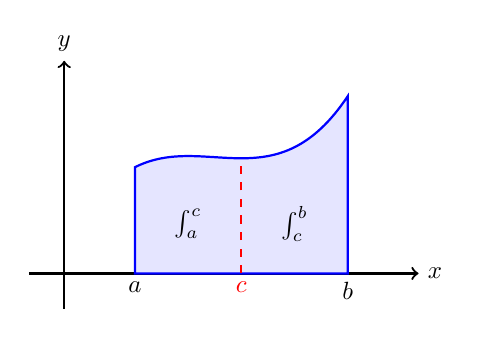
\begin{tikzpicture}[scale=0.9, every node/.style={scale=0.9}]
    \draw[->, thick] (-0.5, 0) -- (5, 0) node[right] {$x$};
    \draw[->, thick] (0, -0.5) -- (0, 3) node[above] {$y$};
    \draw[thick, blue, fill=blue!10] (1,0) -- (1,1.5) .. controls (2,2) and (3,1) .. (4,2.5) -- (4,0) -- cycle;
    \draw[dashed, thick, red] (2.5, 0) -- (2.5, 1.55);
    \node[below] at (1, 0) {$a$};
    \node[below, red] at (2.5, 0) {$c$};
    \node[below] at (4, 0) {$b$};
    \node at (1.75, 0.7) {$\int_a^c$};
    \node at (3.25, 0.7) {$\int_c^b$};
\end{tikzpicture}
\end{center}
\vspace{0.5em}

\begin{proof}
Функция интегрируема по критерию Дарбу $\iff \forall \varepsilon > 0 \,\, \exists T: S(T) - s(T) < \varepsilon$.

\paragraph{1. Необходимость ($\implies$)} 
Пусть $f \in \mathcal{R}[a, b]$. Зафиксируем $\varepsilon > 0$. Существует разбиение $T$, где $S(T) - s(T) < \varepsilon$.
Добавим в $T$ точку $c$ (если её там нет), получим измельченное разбиение $T^* = T \cup \{c\}$. При измельчении разность сумм Дарбу только уменьшается: $S(T^*) - s(T^*) \le S(T) - s(T) < \varepsilon$.
Разбиение $T^*$ распадается на $T_1$ (для $[a, c]$) и $T_2$ (для $[c, b]$). Суммы Дарбу складываются линейно:
$$ (S(T_1) - s(T_1)) + (S(T_2) - s(T_2)) = S(T^*) - s(T^*) < \varepsilon $$
Так как обе скобки $\ge 0$, каждая из них строго меньше $\varepsilon$. По критерию Дарбу, $f \in \mathcal{R}[a, c]$ и $f \in \mathcal{R}[c, b]$.

\paragraph{2. Достаточность ($\impliedby$)}
Пусть $f \in \mathcal{R}[a, c]$ и $f \in \mathcal{R}[c, b]$. Для $\varepsilon > 0$ существуют разбиения $T_1$ и $T_2$, такие что разность сумм для каждого меньше $\frac{\varepsilon}{2}$.
Объединим их в общее разбиение $T = T_1 \cup T_2$. Точка $c$ автоматически станет узлом.
$$ S(T) - s(T) = (S(T_1) - s(T_1)) + (S(T_2) - s(T_2)) < \frac{\varepsilon}{2} + \frac{\varepsilon}{2} = \varepsilon $$
По критерию Дарбу $f(x)$ интегрируема на всем $[a, b]$.

\paragraph{3. Вывод равенства}
Рассмотрим интегральную сумму $\sigma_{[a,b]}$ для разбиения, содержащего узел $c$. Она строго распадается на две части: $\sigma_{[a,b]} = \sigma_{[a,c]} + \sigma_{[c,b]}$. Переходя к пределу при $\lambda(T) \to 0$, получаем $\int_a^b = \int_a^c + \int_c^b$.
\end{proof}


% --- Для Вопроса 17 (Аддитивность) ---
\begin{tcolorbox}[colback=gray!5, colframe=black, boxrule=0.5pt, arc=0pt]
\textbf{Резюмируем (Аддитивность):} \\
\textbf{Тезис:} $\int_a^c f dx = \int_a^b f dx + \int_b^c f dx$. \\
\textbf{Ход:} Выбираем специальное разбиение $T$ такое, что точка $b$ — обязательный узел разбиения. \\
\textbf{Разбиение:} $T_1 = \{x_0, \dots, b\}$ для $[a,b]$ и $T_2 = \{b, \dots, x_n\}$ для $[b,c]$. \\
\textbf{Сумма:} $\sigma(T) = \sum_{x_i \le b} f(\xi_i)\Delta x_i + \sum_{x_i > b} f(\xi_i)\Delta x_i = \sigma(T_1) + \sigma(T_2)$. \\
\textbf{Финал:} При $\lambda \to 0$ обе части стремятся к своим интегралам, сумма остается равенством.
\end{tcolorbox}


% --- Вопрос 18 ---
\examquestion{18}{Свойства-неравенства для определенного интеграла}
{Сформулируйте и строго докажите теорему об оценке модуля интеграла через интеграл от модуля. Докажите также вспомогательное утверждение: если $f\in\mathcal{R}[a,b]$, то и $|f|\in\mathcal{R}[a,b]$.}

\paragraph{Суть на пальцах}
Интеграл (без модуля) считает площадь с учетом знака. То есть области под осью $X$ идут со знаком минус и съедают часть положительной площади (это «перемещение» вперед-назад). А интеграл от модуля $|f(x)|$ воспринимает все площади как положительные (он отзеркаливает "нижние" куски наверх — это весь пройденный «путь»). Очевидно, что суммарный путь $\ge$ итогового перемещения.

\vspace{0.5em}
\begin{center}
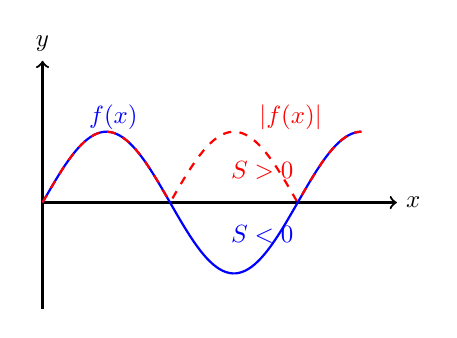
\begin{tikzpicture}[scale=0.9, every node/.style={scale=0.9}]
    \draw[->, thick] (0, 0) -- (5, 0) node[right] {$x$};
    \draw[->, thick] (0, -1.5) -- (0, 2) node[above] {$y$};
    \draw[thick, blue, domain=0:4.5, samples=100] plot (\x, {sin(\x*100)});
    \draw[thick, red, dashed, domain=0:4.5, samples=100] plot (\x, {abs(sin(\x*100))});
    \node[blue] at (1, 1.2) {$f(x)$};
    \node[red] at (3.5, 1.2) {$|f(x)|$};
    \node[below, blue] at (3.1, -0.2) {$S < 0$};
    \node[above, red] at (3.1, 0.2) {$S > 0$};
\end{tikzpicture}
\end{center}
\vspace{0.5em}

\paragraph{1. Доказательство леммы ($f \in \mathcal{R} \implies |f| \in \mathcal{R}$)}
\begin{proof}
Для любых точек $x, y$ на отрезке по неравенству треугольника: $\big| |f(x)| - |f(y)| \big| \le |f(x) - f(y)|$.
Это значит, что максимальный размах (колебание) функции с модулем не превосходит колебания оригинальной функции: $\omega_i(|f|) \le \omega_i(f)$.
Умножим на $\Delta x_i$ и просуммируем:
$$ S(|f|, T) - s(|f|, T) \le S(f, T) - s(f, T) $$
По условию $f \in \mathcal{R}$, значит правая часть меньше $\varepsilon$. Значит, и левая меньше $\varepsilon$. По критерию Дарбу $|f| \in \mathcal{R}$.
\end{proof}

\paragraph{2. Доказательство основного неравенства}
\begin{proof}
Запишем интегральную сумму для $f(x)$. Применим школьное неравенство треугольника ($|A+B| \le |A|+|B|$):
$$ \left| \sigma(f, T, \xi) \right| = \left| \sum_{i=1}^n f(\xi_i)\Delta x_i \right| \le \sum_{i=1}^n |f(\xi_i)|\Delta x_i = \sigma(|f|, T, \xi) $$
При предельном переходе $\lambda(T) \to 0$ нестрогое неравенство сохраняется:
$$ \left| \int_a^b f(x) dx \right| \le \int_a^b |f(x)| dx $$
\end{proof}

% --- Для Вопроса 18 (Монотонность) ---
\begin{tcolorbox}[colback=gray!5, colframe=black, boxrule=0.5pt, arc=0pt]
\textbf{Резюмируем (Монотонность):} \\
\textbf{Тезис:} Если $f(x) \le g(x)$ на $[a,b]$, то $\int_a^b f dx \le \int_a^b g dx$. \\
\textbf{Доказательство:} Рассмотрим $h(x) = g(x) - f(x)$. По условию $h(x) \ge 0$. \\
\textbf{Следствие:} Из доказанного ранее свойства "сохранения знака" (вопрос 16) имеем $\int_a^b h(x) dx \ge 0$. \\
\textbf{Финал:} В силу линейности $\int_a^b (g - f) dx = \int_a^b g dx - \int_a^b f dx \ge 0$, откуда $\int_a^b g dx \ge \int_a^b f dx$.
\end{tcolorbox}

% --- Вопрос 19 ---
\examquestion{19}{Первая теорема о среднем значении}
{Сформулируйте первую теорему о среднем значении. Проведите её доказательство для непрерывной функции $f(x)$. Дайте геометрическую интерпретацию.}

\paragraph{Суть на пальцах (Геометрическая интерпретация)}
Представь, что график функции — это неровная гора песка на фундаменте $[a,b]$. Если проехаться по этой горе бульдозером и идеально выровнять песок, то получится плоский прямоугольник точно такой же площади и ширины. 
Высота этого прямоугольника и есть «среднее значение». Теорема гарантирует: так как функция непрерывна (без разрывов), реальная высота горы в какой-то точке $\xi$ обязательно совпадет с высотой этого выровненного прямоугольника.

\vspace{0.5em}
\begin{center}
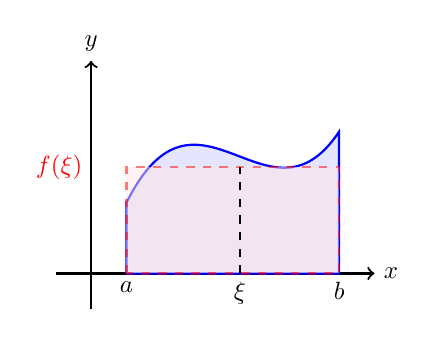
\begin{tikzpicture}[scale=0.9, every node/.style={scale=0.9}]
    \draw[->, thick] (-0.5, 0) -- (4, 0) node[right] {$x$};
    \draw[->, thick] (0, -0.5) -- (0, 3) node[above] {$y$};
    % Кривая
    \draw[thick, blue, fill=blue!10] (0.5,0) -- (0.5, 1) .. controls (1.5, 3) and (2.5, 0.5) .. (3.5, 2) -- (3.5,0) -- cycle;
    % Прямоугольник
    \draw[thick, red, dashed, fill=red!10, opacity=0.5] (0.5,0) rectangle (3.5, 1.5);
    \draw[dashed, thick] (2.1, 0) -- (2.1, 1.5);
    \node[below] at (0.5, 0) {$a$};
    \node[below] at (3.5, 0) {$b$};
    \node[below] at (2.1, 0) {$\xi$};
    \node[left, red] at (0, 1.5) {$f(\xi)$};
\end{tikzpicture}
\end{center}
\vspace{0.5em}

\paragraph{Формулировка и доказательство теоремы}
Если функция $f(x)$ непрерывна на $[a, b]$, то существует точка $\xi \in [a, b]$, такая что: $\int_a^b f(x) dx = f(\xi)(b - a)$.
\begin{proof}
1. $f(x) \in \mathcal{C}[a, b]$. По теореме Вейерштрасса функция достигает минимума $m$ и максимума $M$: $m \le f(x) \le M$.
2. Проинтегрируем неравенство по всему отрезку $[a, b]$:
$$ \int_a^b m \, dx \le \int_a^b f(x) dx \le \int_a^b M \, dx \implies m(b-a) \le \int_a^b f(x) dx \le M(b-a) $$
3. Разделим на длину отрезка $(b - a) > 0$:
$$ m \le \frac{1}{b - a} \int_a^b f(x) dx \le M $$
4. Обозначим центральную дробь за $\mu$. Видим, что $\mu$ лежит между $m$ и $M$.
5. По теореме Коши о промежуточном значении, непрерывная функция $f(x)$ обязана принимать любое значение между своим минимумом и максимумом. Значит, существует точка $\xi \in [a, b]$, в которой $f(\xi) = \mu$.
6. Подставив $f(\xi)$ в формулу, получаем: $\int_a^b f(x) dx = f(\xi)(b - a)$.
\end{proof}


% --- Для Вопроса 19 (Оценка интеграла) ---
\begin{tcolorbox}[colback=gray!5, colframe=black, boxrule=0.5pt, arc=0pt]
\textbf{Резюмируем (Оценка):} \\
\textbf{Тезис:} $m(b-a) \le \int_a^b f(x) dx \le M(b-a)$, где $m, M$ — глобальные inf/sup. \\
\textbf{Ход:} Для любого разбиения $m \le f(\xi_i) \le M$. \\
\textbf{Суммирование:} $m \Delta x_i \le f(\xi_i) \Delta x_i \le M \Delta x_i$. Суммируем по всем $i$: \\
$m \sum \Delta x_i \le \sigma \le M \sum \Delta x_i$. \\
\textbf{Финал:} Так как $\sum \Delta x_i = b-a$, получаем $m(b-a) \le \sigma \le M(b-a)$. Предельный переход сохраняет неравенства.
\end{tcolorbox}



% --- Вопрос 20 ---
\examquestion{20}{Обобщенная теорема о среднем}
{Сформулируйте и докажите обобщенную теорему о среднем для функций $f,g\in\mathcal{R}[a,b]$. Обоснуйте роль условия знакопостоянства $g(x)$. Приведите аналитический контрпример при нарушении этого условия.}

\paragraph{Суть на пальцах}
В первой теореме (№19) мы искали обычное среднее значение. Обобщенная теорема ищет взвешенное среднее. 
Функция $g(x)$ работает как веса. Если веса меняют знак (то в плюс, то в минус), они могут взаимно уничтожиться, и сумма станет нулем. 
Тогда появится деление на ноль, и всё сломается. Поэтому $g(x)$ строго обязана не менять знак: быть везде $\ge 0$ или везде $\le 0$.

Разница наглядно: в обычной теореме мы заменяем площадь под графиком $f(x)$ на простой прямоугольник. В обобщенной мы делаем то же самое, но с учетом "плотности" $g(x)$. Если плотность на отрезке разная, то и среднее значение (наш $\mu$) сместится в ту сторону, где вес больше.

\paragraph{Формулировка и доказательство}
Пусть $f, g \in \mathcal{R}[a, b]$, и пусть $g(x)$ знакопостоянна (для определенности $g(x) \ge 0$). Тогда существует число $\mu \in [\inf f, \sup f]$, такое что:
$$ \int_a^b f(x)g(x)dx = \mu \int_a^b g(x)dx $$
Если $f(x)$ непрерывна, то $\mu = f(\xi)$.

\begin{proof}
1. Функция $f(x)$ ограничена своими точными гранями: $m \le f(x) \le M$.
2. Умножим это неравенство на $g(x)$. Так как $g(x) \ge 0$, знаки неравенства сохраняются. Если бы $g(x)$ меняла знак, неравенство бы разрушилось.
$$ m \cdot g(x) \le f(x)g(x) \le M \cdot g(x) $$
3. Интегрируем на $[a, b]$:
$$ m \int_a^b g(x)dx \le \int_a^b f(x)g(x)dx \le M \int_a^b g(x)dx $$
4. Если интеграл весов $\int_a^b g(x)dx = 0$, то центральный интеграл тоже $0$. Теорема верна при любом $\mu$. 
5. Если $\int_a^b g(x)dx > 0$, разделим на него всё неравенство:
$$ m \le \frac{\int_a^b f(x)g(x)dx}{\int_a^b g(x)dx} \le M $$
Дробь по центру - это некоторое число $\mu \in [m, M]$. Если $f$ непрерывна, по теореме Коши она принимает это значение в некоторой точке $\xi$, то есть $f(\xi) = \mu$.
\end{proof}

\paragraph{Графический смысл (обычное среднее)}
Площадь под кривой равна площади заштрихованного прямоугольника.
\begin{center}
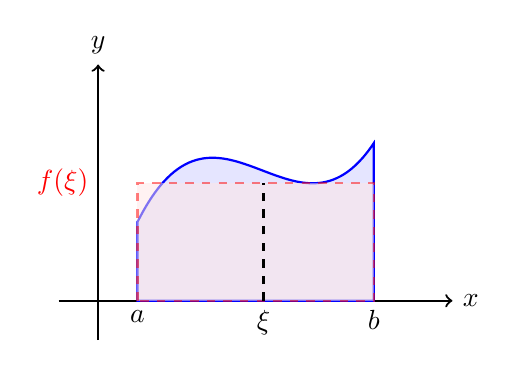
\begin{tikzpicture}
    % Оси
    \draw[->, thick] (0, -0.5) -- (0, 3) node[above] {$y$};
    \draw[->, thick] (-0.5, 0) -- (4.5, 0) node[right] {$x$};
    % Кривая
    \draw[thick, blue, fill=blue!10] (0.5,0) -- (0.5, 1) .. controls (1.5, 3) and (2.5, 0.5) .. (3.5, 2) -- (3.5,0) -- cycle;
    % Прямоугольник
    \draw[thick, red, dashed, fill=red!10, opacity=0.5] (0.5,0) rectangle (3.5, 1.5);
    \draw[dashed, thick] (2.1, 0) -- (2.1, 1.5);
    \node[below] at (0.5, 0) {$a$};
    \node[below] at (3.5, 0) {$b$};
    \node[below] at (2.1, 0) {$\xi$};
    \node[left, red] at (0, 1.5) {$f(\xi)$};
\end{tikzpicture}
\end{center}

\paragraph{Аналитический контрпример (почему без знакопостоянства всё ломается)}
Рассмотрим отрезок $[-1, 1]$. Пусть $f(x) = x$ и $g(x) = x$. 
Тут функция "весов" $g(x)$ меняет знак в нуле.
1. Считаем левую часть:
$$ \int_{-1}^{1} f(x)g(x)dx = \int_{-1}^{1} x^2 dx = \left[ \frac{x^3}{3} \right]_{-1}^{1} = \frac{2}{3} $$
2. Считаем интеграл весов (правую часть):
$$ \int_{-1}^{1} g(x)dx = \int_{-1}^{1} x dx = \left[ \frac{x^2}{2} \right]_{-1}^{1} = 0 $$
3. Подставляем в формулу теоремы:
$$ \frac{2}{3} = \mu \cdot 0 \implies \frac{2}{3} = 0 $$
Абсурд. Без жесткого условия знакопостоянства теорема ложна.


% --- Для Вопроса 20 (Теорема о среднем) ---
\begin{tcolorbox}[colback=gray!5, colframe=black, boxrule=0.5pt, arc=0pt]
\textbf{Резюмируем (Теорема о среднем):} \\
\textbf{Тезис:} $\exists \xi \in [a,b]: \int_a^b f(x) dx = f(\xi)(b-a)$. \\
\textbf{Ход:} 1) Из оценки (вопрос 19) делим на $(b-a)$: $m \le \frac{1}{b-a} \int_a^b f(x) dx \le M$. \\
2) Пусть $\mu = \frac{1}{b-a} \int_a^b f(x) dx$. Число $\mu$ лежит между min и max функции. \\
3) По теореме Коши (о промежуточном значении непрерывной функции), $\exists \xi$, что $f(\xi) = \mu$. \\
4) Умножаем обратно на $(b-a)$ — готово.
\end{tcolorbox}